% Three-model comparison figure: Legacy OS, In-Process Isolation, Confidential VM
% Assumes \usepackage{tikz}, \usepackage{subcaption}, and \usetikzlibrary{positioning, calc, matrix}

\def\boxwidth{4.0cm}
\def\boxheight{0.8cm}
\pgfmathsetlengthmacro{\appwidth}{\boxwidth/3 - 0.3cm}

\tikzstyle{tcb}=[rectangle,draw,align=center,minimum width=\boxwidth,text width=\boxwidth,minimum height=\boxheight,fill=blue!20]
\tikzstyle{file}=[rectangle,draw,fill=green!20,minimum width=0.8cm,
minimum height=0.5cm,font=\scriptsize]
\tikzstyle{proc}=[rectangle,draw,fill=red!20,minimum width=\appwidth,minimum height=\boxheight,font=\scriptsize]
\tikzstyle{boundary}=[draw=blue,very thick]
% -------------------------------------------------------------
% (a) Legacy OS protection
% -------------------------------------------------------------
\begin{subfigure}[t]{0.31\textwidth}
	\centering
	\begin{tikzpicture}[node distance=1.1cm]
		\node[
			draw=green, very thick, fill=green!20,
			minimum width=4cm,minimum height=3cm
		](sys){};
		\node[
			draw=blue, very thick, fill=blue!20,
			minimum width=3.7cm,minimum height=2.7cm
		] (os) at (sys) {};
		\node[
			draw=red, very thick, fill=red!20,
			minimum width=3.4cm,minimum height=2.4cm
		] (hw) at (os) {};



		% \matrix[column sep=0pt,row sep=5pt] {
		%
		% 	\node[tcb, text height =1.0 cm] (os) {Operating System}; \\
		% 	\node[tcb] (hw) {Hardware (CPU, Memory)};                \\
		% };
		%
		% \matrix (apps) [above of=os, column sep=7pt,yshift=0.3cm] {
		% 	\node[proc] (p1) {Proc. 1}; &
		% 	\node[proc] (p2) {Proc. 2}; &
		% 	\node[proc] (p3) {Proc. 3};   \\
		% };
		% % Files below OS
		% \node[file, below of=p1,yshift=-.0cm] (f1) {File 1};
		% \node[file, below of=p2,yshift=-.0cm] (f2) {File 2};
		% \node[file, below of=p3,yshift=-.0cm] (f3) {File 3};
		%
		% \node[boundary,fit=(p1)(f1),inner sep=2pt] (b1) {};
		% \node[boundary,fit=(p2)(f2),inner sep=2pt] (b2) {};
		% \node[boundary,fit=(p3)(f3),inner sep=2pt] (b3) {};
		% \node[boundary,fit=(p3)(f3),inner sep=2pt] (b3) {};
		%
		% Kernel boundary
		% \draw[boundary] ($(os.north west)+(-0.0,0.15)$) -- ($(os.north east)+(0.0,0.15)$);

		% Legend
		% \matrix [draw, above of=apps, yshift=1.5cm, xshift=5cm, column sep=6pt, row sep=2pt] {
		% Trusted
		% \node[rectangle,draw,fill=blue!20,minimum width=0.4cm,minimum height=0.4cm] {};  &
		% \node[anchor=west] {Trusted};                                                    &
		% % Untrusted
		% \node[rectangle,draw,fill=red!20,minimum width=0.4cm,minimum height=0.4cm] {};   &
		% \node[anchor=west] {Untrusted};                                                  &
		%
		% % Object (File)
		% \node[rectangle,draw,fill=green!20,minimum width=0.4cm,minimum height=0.4cm] {}; &
		% \node[anchor=west] {System Resources};                                             \\
		%
		% \node {\begin{tikzpicture}\draw[boundary] (0,0) -- (0.6,0);\end{tikzpicture}};
		%                                                                                  &
		% \node[anchor=west] {Domain boundary};                                              \\
		% };
	\end{tikzpicture}
	\caption{Legacy OS protection introduces protection domains for user processes and kernel.}\label{legacy-align}

\end{subfigure}\hfil
\begin{subfigure}[t]{0.31\textwidth}

	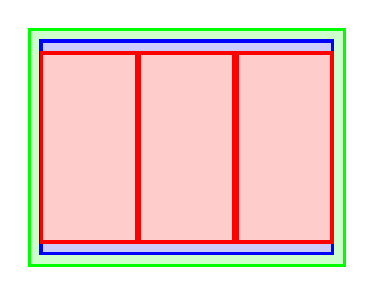
\begin{tikzpicture}[node distance=1.1cm]
		\node[
			draw=green, very thick, fill=green!20,
			minimum width=4cm,minimum height=3cm
		](sys){};
		\node[
			draw=blue, very thick, fill=blue!20,
			minimum width=3.7cm,minimum height=2.7cm
		] (os) at (sys) {};
		\matrix[ ] (hw) at (os) {
			\node[draw=red, very thick, fill=red!20,
				minimum width=1.2cm,minimum height=2.4cm
			](){}; &
			\node[draw=red, very thick, fill=red!20,
				minimum width=1.2cm,minimum height=2.4cm
			](){}; &
			\node[draw=red, very thick, fill=red!20,
				minimum width=1.2cm,minimum height=2.4cm
			](){}; \\
		};

	\end{tikzpicture}
	% \begin{tikzpicture}[node distance=1.1cm]
	% 	\node[
	% 		draw=green, very thick, fill=green!20,
	% 		minimum width=4cm,minimum height=3cm
	% 	](sys){};
	% 	\node[
	% 		draw=blue, very thick, fill=blue!20,
	% 		minimum width=3.7cm,minimum height=2.7cm
	% 	] (os) at (sys) {};
	% 	\node[
	% 		draw=red, very thick, fill=red!20,
	% 		minimum width=3.4cm,minimum height=2.4cm
	% 	] (hw) at (os) {};
	% \end{tikzpicture}
	\caption{.}\label{inprocess-align}

\end{subfigure}\hfil
\begin{subfigure}[t]{0.31\textwidth}
	% \begin{tikzpicture}[node distance=1.1cm]
	% 	\node[
	% 		draw=green, very thick, fill=green!20,
	% 		minimum width=4cm,minimum height=3cm
	% 	](sys){};
	% 	\node[
	% 		draw=blue, very thick, fill=blue!20,
	% 		minimum width=3.7cm,minimum height=2.7cm
	% 	] (os) at (sys) {};
	% 	\node[
	% 		draw=red, very thick, fill=red!20,
	% 		minimum width=3.4cm,minimum height=2.4cm
	% 	] (hw) at (os) {};
	%
	% \end{tikzpicture}
	\caption{Confidential virtual machines~\cite{advanced_micro_device_sev_2022,cca,tdx} establish isolated protection domains for entire VMs.}\label{cvm-alignn}
\end{subfigure}

